\subsection{Try Resource}
Como continuação da evolução do mecanismo de exceção de Java 7 introduziu \texttt{try-resource} onde o \texttt{resouce} é um objeto que implemente \texttt{java.lang.AutoCloseable } ou \texttt{java.io.Closeable} e com isso o mecanismo garante o encerramento do recurso com encerramento do \texttt{statement} o que antes de recurso só era capaz utilizando um bloco \texttt{finally}\footnote{\texttt{try-resource} pode utilizar \texttt{catch} e \texttt{finally} de forma igual ao \texttt{try-catch}}.

\begin{lstlisting}[caption={Try sem adoção de resource.}\label{lst:semResource},language=Java]
static String readFirstLineFromFileWithFinallyBlock(String path)
                                                     throws IOException {
    BufferedReader br = new BufferedReader(new FileReader(path));
    try {
        return br.readLine();
    } finally {
        if (br != null) br.close();
    }
}
\end{lstlisting}

\begin{lstlisting}[caption={Try adotando resource.}\label{lst:comResource},language=Java]
static String readFirstLineFromFileWithFinallyBlock(String path)
                                                     throws IOException {
    try ( BufferedReader br = new BufferedReader(new FileReader(path));){
        return br.readLine();
    } 
}
\end{lstlisting}

Este trabalho contribui com a pesquisa para verificar como é a adoção deste recurso, após a realização das análise foram encontrados \num{1616} ocorrências de utilização onde a Figura:~\ref{fig:Try-Resource} demonstra a distribuição por projetos e somente 13 projetos o utilizam totalizando apenas \num{28}\% dos projetos verificados.

\begin{figure}[h]
	\center
	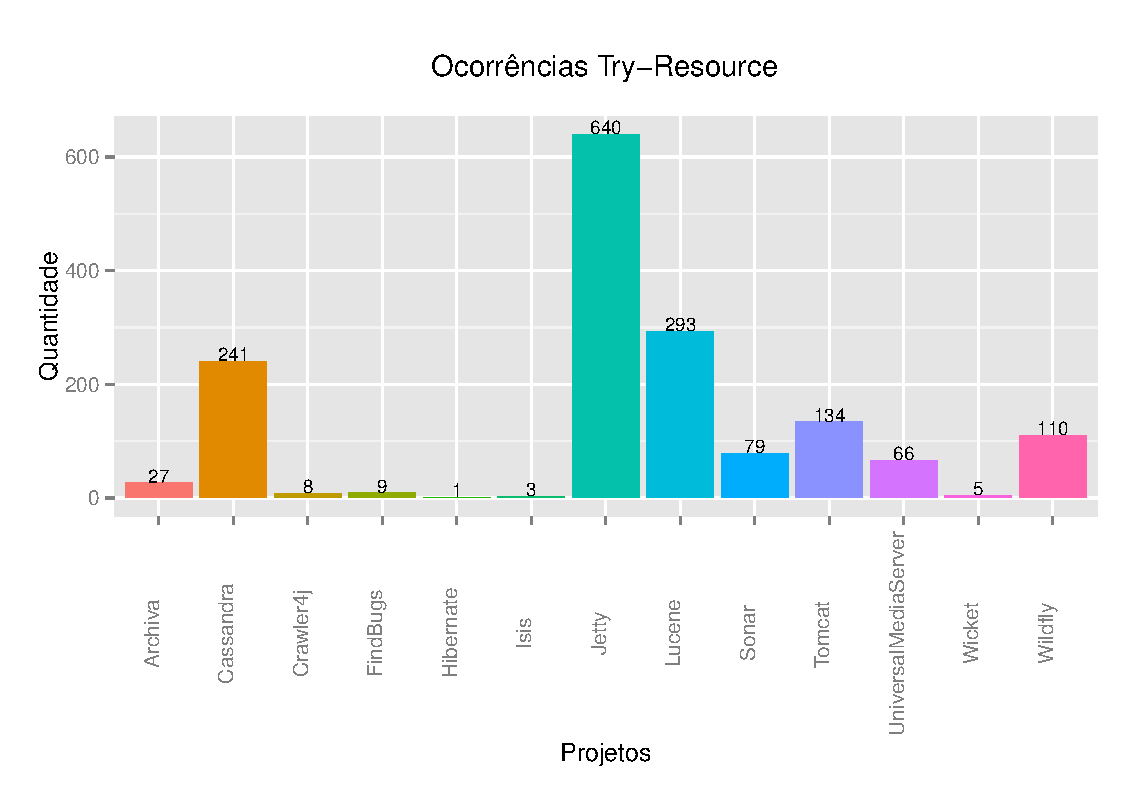
\includegraphics[scale=0.55]{Imagens/ocorrenciasTryResource}
	\label{fig:Try-Resource}
	\caption{Adoção de \texttt{Try-Resource} nos projetos.}
\end{figure}

A Tabela:~\ref{tab:adocaoResource} exibe a distribuição deste recurso por  tipo de sistema. Onde pode-se constatar que os \texttt{Servers-Database} realizaram uma adoção significativa de \num{91}\% em relação aos demais tipos.

\begin{table}[h]
	\centering
	\caption{Adoção Try-Resource por tipo do sistema.}
	\begin{tabular}{cc}
		\hline
		Natureza & Ocorrências \\ 
		\hline \hline
		\texttt{Application} & 115 \\ 
		\texttt{Library} & 17 \\ 
		\texttt{Servers - Database} & 1484 \\ \hline
		\texttt{Total} & 1616 \\ \hline
	\end{tabular}
	\label{tab:adocaoResource} %std means summary of type declarations
\end{table}


